\chapter{Perancangan}
\label{chap:perancangan}
Pada bab ini akan dijelaskan perancangan perangkat lunak yang dibuat pada penelitian ini. Perancangan terdiri dari diagram aktivitas dan masukan perangkat lunak. 

\section{Diagram Aktivitas}
\label{sec:diagramAktivitas}
Perangkat lunak perekaman absen daring otomatis adalah perangkat lunak yang digunakan untuk melakukan absensi secara otomatis bagi mahasiswa UNPAR. Perangkat lunak ini menggunakan Selenium WebDriver sebagai \textit{tools} yang berguna untuk melakukan otomatisasi pada browser web. Perangkat lunak ini juga membutuhkan masukan dari sebuah file konfigurasi untuk menjalankannya.
Diagram Aktivitas untuk perangkat lunak perekaman kehadiran daring otomatis dapat dilihat pada Gambar \ref{fig:diagramActivity}. Berikut ini adalah penjelasan langkah-langkah pada diagram aktifitas:
\begin{enumerate}
	\item Pengguna membuka \textit{file} konfigurasi untuk mengubah \textit{email} UNPAR dan \textit{password} milik pribadi (langkah ini cukup dijalankan sekali saja).
	\item Pengguna membuka aplikasi dan menjalankan aplikasi tersebut.
	\item Perangkat lunak menerima masukan dari file konfigurasi yang sudah disetel.
	\item Perangkat lunak akan membuka browser Google Chrome secara otomatis.
	\item Perangkat lunak akan masuk ke situs \url{https://studentportal.unpar.ac.id/} yang merupakan situs bagi Mahasiswa UNPAR untuk dapat melakukan absensi.
	\item Perangkat lunak akan melakukan \textit{login} secara otomatis dengan \textit{email} dan \textit{password} yang sesuai dari \textit{file} konfigurasi.
	\item Perangkat lunak akan membuka halaman situs untuk melakukan absensi perkuliahan.
	\item Perangkat lunak akan melakukan absensi secara otomatis,
	\item Perangkat lunak akan menutup browser.
\end{enumerate}
\begin{figure}[H]
	\centering
	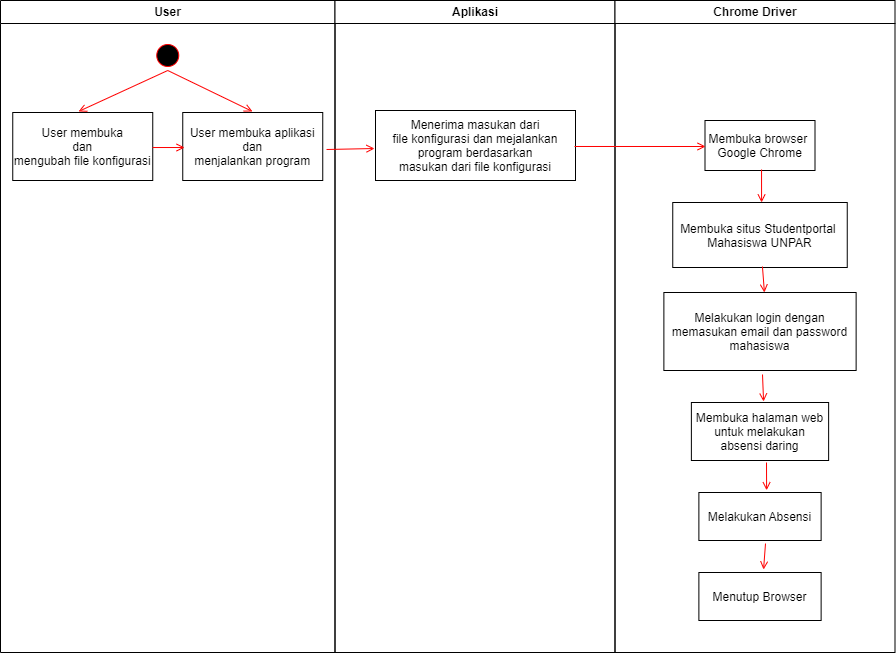
\includegraphics[scale=0.5]{Gambar/diagramActivity.png}
	\caption{Diagram Aktivitas Perangkat Lunak Absen Daring Otomatis} 
	\label{fig:diagramActivity}
\end{figure}

\section{Masukan Perangkat Lunak}
\label{sec:inputConfig} 
Perangkat lunak perekaman kehadiran daring otomatis membutuhkan 1 file sebagai masukan, yaitu \textit{file} .config (\textit{file} konfigurasi). Pada \textit{file} .config, nomor baris sebagai \textit{keys} dan \textit{string} berupa kata yang merupakan fungsi dari Selenium WebDriver dan elemen yang diambil untuk melakukan perekaman kehadiran daring otomatis sebagai \textit{values}. Contoh \textit{file} .config dapat dilihat pada Listing \ref{kode:4:conf}.
\begin{lstlisting}[caption=Contoh \textit{file} .config untuk Masukan Perangkat Lunak Perekaman Kehadiran Daring Otomatis, label=kode:4:conf]
	[database_config]
	1 = open https://studentportal.unpar.ac.id
	2 = click #login-button
	3 = sendkeys #username 2017730035@student.unpar.ac.id 
	4 = quit
\end{lstlisting}
Berikut ini penjelasan dari isi dari contoh \textit{file} .config:
\begin{itemize}
	\item Baris pertama berisi nama \textit{section} untuk isi \textit{file} .config.
	\item \textit{keys} pada \textit{file} .config ini pasti berupa angka yang terurut agar perangkat lunak dapat menjalankannya secara terurut.
	\item Terdapat 4 fungsi kata dari Selenium WebDriver, yaitu \textit{open}, \textit{click}, \textit{sendkeys}, dan \textit{quit}.
	\item \textit{Keys} 1 pasti diisi oleh fungsi \textit{open}, lalu diisi situs web yang ingin dibuka (\url{https://studentportal.unpar.ac.id}), karena langkah pertama setelah berhasil membuka browser adalah menuju pada situs web yang akan diotomatisasi.
	\item \textit{Keys} 2 memiliki fungsi \textit{click} untuk menekan tombol secara otomatis dan diisi elemen ``\#login-button'' yang diambil berdasarkan CSS Selector.
	\item \textit{Keys} 3 memiliki fungsi \textit{sendkeys} untuk memasukan suatu nilai ke dalam elemen yang dipilih, yaitu elemen ``\#username'' dan isinya adalah ``2017730035@student.unpar.ac.id''.
	\item \textit{Keys} 4 memiliki fungsi \textit{quit} untuk menutup browsernya.
\end{itemize}
Elemen yang dipakai dalam \textit{file} .config ini diambil dengan cara melakukan \textit{inspect element} pada web yang ingin dilakukan otomatisasi. Pada Gambar \ref{fig:inspect} adalah cara yang dilakukan untuk mendapat elemen yang ingin digunakan untuk melakukan otomatisasi. Untuk mendapatkan elemen tersebut, perlu melakukan klik kanan pada bagian elemen yang ingin diambil, lalu pilih ``inspect''. Setelah melakukan ``inspect'' maka akan muncul dokumen HTML yang dapat dilihat pada bagian kanan Gambar \ref{fig:inspect}, sehingga dapat melakukan pengambilan elemen yang diperlukan.
\begin{figure}[H]
	\centering
	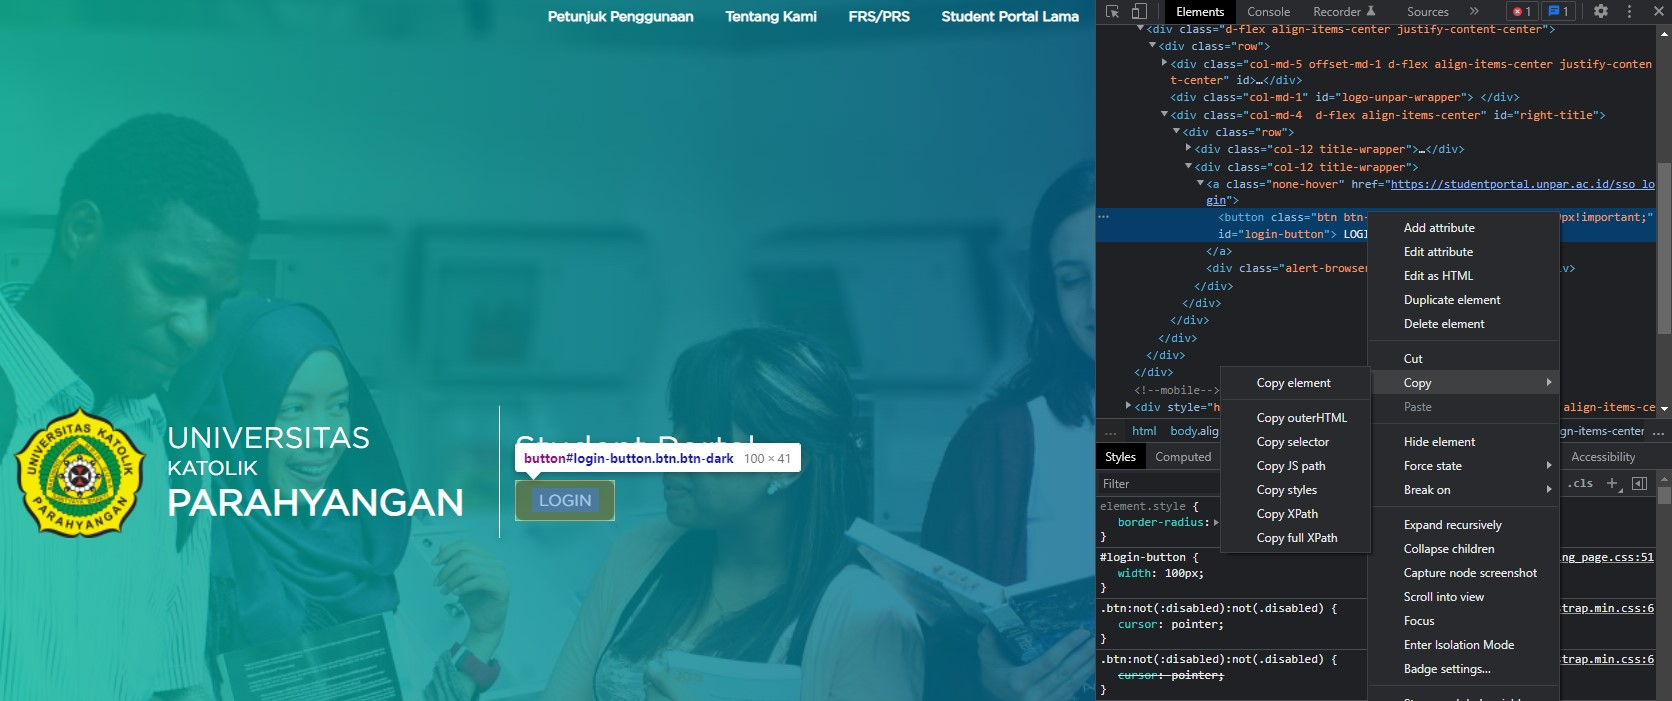
\includegraphics[scale=0.4]{Gambar/elemen.jpg}
	\caption{Tampilan Melakukan \textit{Inspect Element}} 
	\label{fig:inspect}
\end{figure}	